\chapter{\sffamily Managing a rugby match}

{\bfseries\sffamily Concept.} Building a toy model simulation of a rugby match whose outcome can be manipulated through correctly-timed player substitutions and game management decisions. The dexetera state manipulation framework we have built around the stochadex can meet these requirements, and a dashboard can be created for user interaction. All this combines together to make a simple dashboard game, which we call: `trywizard'. For the mathematically-inclined, this chapter will motivate the construction of a specific modelling framework for rugby match simulation. For the programmers, the public Git repository for the code described in this chapter can be found here: \href{https://github.com/umbralcalc/trywizard}{https://github.com/umbralcalc/trywizard}.

\section{\sffamily Designing the event simulation engine}

Since the basic state manipulation framework and simulation engine will run using \href{https://github.com/umbralcalc/dexetera}{dexetera}, the mathematical novelties in this project are all in the design of the rugby match model itself. And, as ever, we're not especially keen on spending a lot of time doing detailed data analysis to come up with the most realistic values for the parameters that are dreamed up here. Even though this would also be interesting.\footnote{One could do this data analysis, for instance, by scraping player-level performance data from one of the excellent websites that collect live commentary data such as \href{https://www.rugbypass.com/}{rugbypass.com} or \href{https://www.espn.co.uk/rugby/}{espn.co.uk/rugby}.}

Let's begin by specifying an appropriate state space to live in when simulating a rugby match. It is important at this level that events are defined in quite broadly applicable terms, as it will define the state space available to our stochastic sampler and hence the simulated game will never be allowed to exist outside of it. It seems reasonable to characterise a rugby union match by the following set of states: {\sf Penalty}, {\sf Free Kick} (the punitive states); {\sf Penalty Goal}, {\sf Drop Goal}, {\sf Try} (the scoring states); {\sf Kick Phase}, {\sf Run Phase}, {\sf Knock-on}, {\sf Scrum}, {\sf Lineout}, {\sf Maul} and {\sf Ruck} (the general play states). Using this set of states, in Fig.~\ref{fig:event-graph} we have summarised our approach to match state transitions into a single event graph. In order to capture the fully detailed range of events that are possible in a real-world match, we've needed to be a little imaginative in how we define the kinds of state transitions which occur. In other words; it's fair to say that our simplified model here represents just a subset of states that a real rugby match could exist in.

\begin{figure}[h]
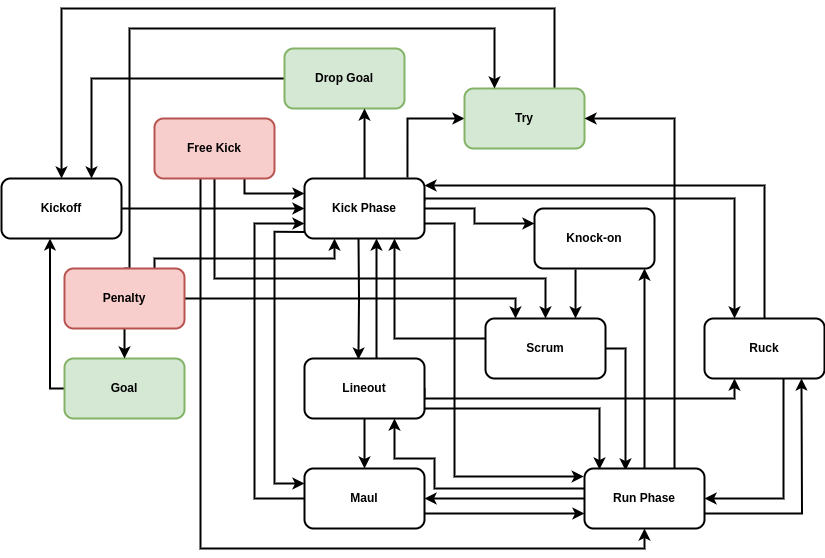
\includegraphics[width=14cm]{images/trywizard-event-graph.drawio.png}
\caption{Simplified event graph of a rugby union match.}
\label{fig:event-graph}
\end{figure}

In addition to occupying some state in the event graph, the state of a rugby match must also include a binary `possession' element which encodes which team has the ball at any moment. We should also include the 2-dimensional pitch location of the ball as an element of the match state in order to get a better sense of how likely some state transitions are, e.g., when playing on the edge of the pitch near the touchline it's clearly more likely that a {\sf Run Phase} is going to result in a {\sf Lineout} than if the state is currently in the centre of the pitch. To add even more detail, in the next section we will elaborate further by introducing states for each playing position on each side, which encode the playing abilities of each player, their fatigue status and their substitution status. The latter of these keeps track of whether or not the player has been injured or yellow/red-carded during the course of a game and should also enable management strategies to become more nuanced.

Since a rugby match exists in continuous time, it is natural to choose a continuous-time event-based simulation model for our game engine. As we have discussed in previous chapters already, this means we will be characterising transition probabilities of the event graph in Fig.~\ref{fig:event-graph} by ratios of event rates in time. Recalling our notation in previous chapters, if we consider the current state vector of the match $X_{\sf t}$, we can start by assigning each transition $a\rightarrow b$ on the event graph an associated rate of occurance $\lambda_{a\rightarrow b} (X_{\sf t}, {\sf t})$ which is defined in units of continuous time, e.g., seconds. In addition to the transitions displayed on the graph, we can add a `possession change transition'; where the possession of the ball in play moves to the opposing team. This transition may occur while the match is also in any of the white-coloured states on the graph and let's assign this a time and state-dependent expected rate of occurance $\lambda_{\rm pos}(X_{\sf t}, {\sf t})$.

Based on our dicussion above, an appropriate encoding for the overall game state at timestep index ${\sf t}$ could be a state vector $X_{{\sf t}}$ whose elements are
%%
\begin{align}
X^0_{{\sf t}}&=\begin{cases} 0 & \text{Match State} = \text{{\sf Penalty}}\\ 1 & \text{Match State} = \text{{\sf Free Kick}} \\ \dots & \end{cases} \\
X^1_{{\sf t}}&=\begin{cases} 0 & \text{Possession} = \text{{\sf Home Team}}\\ 1 & \text{Possession} = \text{{\sf Away Team}} \end{cases} \,.
\end{align}
%%
But how does this overall game state connect to the event rates? The probabilistic answer is quite straightforward. If the probability of the match state being $X^0_{{\sf t}}=a$ at timestep ${\sf t}$ is written as $P^0_{{\sf t}}(a)$, then the probability of $X^0_{{\sf t}+1}=b$ in the following timestep is
%%
\begin{align}
P^0_{{\sf t}+1}(b) = \frac{\lambda_{a\rightarrow b} (X_{\sf t}, {\sf t})P^0_{{\sf t}}(a)}{\big[ \frac{1}{\tau} + \sum_{\forall b}\lambda_{a\rightarrow b} (X_{\sf t}, {\sf t})\big] P^0_{{\sf t}}(a)} \label{eq:match-state-transition-probs}\,,
\end{align}
%%
where $\forall b$ in the summation indicates that all the available transitions from $a$ should be summed over. Note that, in the expression above, we have also defined $\tau$ as a timescale short enough such that no transition is likely to occur during that interval. 

Before we move on to other details, it's quite important to recognise that because our process is defined in continuous time, the event rates may well vary continuously (this will be especially true when we talk about, e.g., player fatigue). Hence, Eq.~(\ref{eq:match-state-transition-probs}) is only an \emph{approximation} of the true underlying dynamics that we are trying to simulate --- and this approximation will only be accurate if $\tau$ is small. The reader may recall that we discussed this same issue from the point of view of simulating time-inhomogeneous Poisson processes with the rejection method when we were building the stochadex in an earlier chapter. 

An equivalent to Eq.~(\ref{eq:match-state-transition-probs}) should also apply to the possession change transition rate, i.e., the probability that the {\sf Home Team} has possession $P^1_{{\sf t}}$ at time ${\sf t}$ evolves according to
%%
\begin{align}
P^1_{{\sf t}+1} = \frac{\lambda_{\rm pos} (X_{\sf t}, {\sf t})(1-P^1_{{\sf t}})}{\big[ \frac{1}{\tau} + \lambda_{\rm pos} (X_{\sf t}, {\sf t})\big] (1-P^1_{{\sf t}})} \label{eq:possession-change-probs}\,.
\end{align}
%%

While these match state transitions and possession changes are taking place, we also need to come up with a model for how the ball location $L_{{\sf t}}$ changes during the course of a game, and as a function of the current game state. If we associate every state on the event graph with a single change in spatial location of the ball on the pitch, we then need to construct a process which makes `jumps' in 2-dimensional space each time a state transition occurs. For the sake of simplicity, we will choose this model to just be a 2-dimensional Gaussian distribution such that the probability density $P_{{\sf t}}(\ell )$ of $L_{{\sf t}}=\ell$ at timestep ${\sf t}$ evolves according to
%%
\begin{align}
P_{{\sf t}+1}(\ell ) = {\sf MultivariateNormalPDF}[\ell ; L_{{\sf t}}, C(X_{{\sf t}}, {\sf t})] \,,
\end{align}
%%
where $C(X_{{\sf t}}, {\sf t})$ is some spatial covariance matrix which depends on the current state and timestep. Note that because $L_{{\sf t}}$ is a part of the overall game state, it will be included as information contained within some elements of $X_{{\sf t}}$ as well. To make this explicit, we can simply set $X^2_{{\sf t}}=L^{\rm lon}_{{\sf t}}$ and $X^3_{{\sf t}}=L^{\rm lat}_{{\sf t}}$ --- where $(L^{\rm lon}_{{\sf t}}, L^{\rm lat}_{{\sf t}})$ denote the longitudinal (lengthwise along the pitch) and lateral (widthwise across the pitch) components of the ball location, respectively.

\section{\sffamily Associating events to player states and abilities}

In the last section we introduced a continuous-time event-based simulation model for a rugby union match. In this section we are going to add more detail into this model by inventing how to associate specific player states and abilities to the event rates of the simulation. Before continuing, we want to reiterate that this model is entirely made up and, while we hope it illustrates some interesting mathematical modelling ideas in the context of rugby, there's no particular reason why a statistical inference with a reliable dataset should prefer our model to others which may exist. In other words, this toy model is just for fun!

\begin{figure}[h]
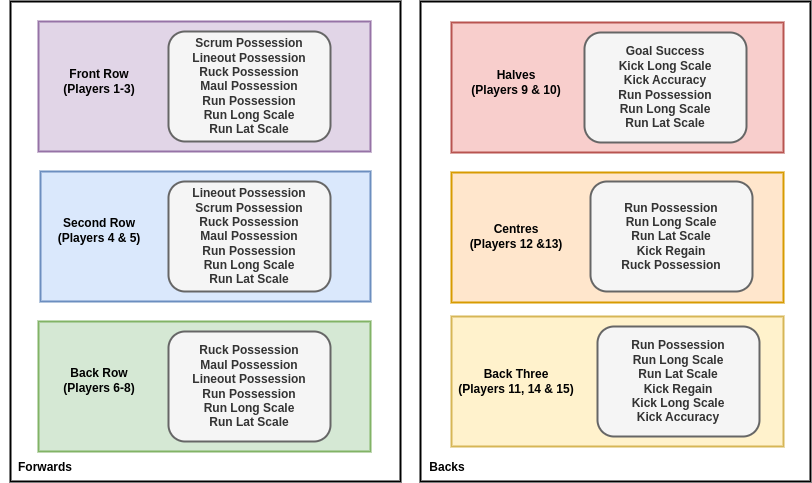
\includegraphics[width=15cm]{images/rugby-player-abilities.drawio.png}
\caption{Associated playing abilities for each position type.}
\label{fig:player-abilities}
\end{figure}

In Fig.~\ref{fig:player-abilities} we have begun by separating playing positions on the rugby field into their usual descriptions and then associating each player type with a short list of simplified attributes. Our model is then to associate a player with an `attacking' and `defensive' ability which corresponds to each of their attributes. For example, a Front Row Forward will have 8 abilities associated to them: 2 for each of their {\sf Scrum}, {\sf Lineout}, {\sf Ruck} and {\sf Maul} attributes. 

Let's now create a vector-valued function $o (a, X^1_{\sf t})$ which returns all of the attacking attributes associated to match state $a$ and an analogous one $d (a, X^1_{\sf t})$ for the defensive attributes. The dependencies of these functions on the ball possession state $X^1_{\sf t}$ comes from the fact that when, e.g., the {\sf Home Team} has possession of the ball it will be their attacking attributes that are returned by $o (a, X^1_{\sf t})$ and the {\sf Away Team}'s defensive attributes that are returned by $d (a, X^1_{\sf t})$. On the other hand, it should be the other team's attributes that are returned by each function when possession is given to the {\sf Away Team}. 

There are different transition types, but thinking of equations of the form...
%%
\begin{align}
\lambda_{a\rightarrow b}(X_{\sf t}, {\sf t}) = \sum_{\forall i} o^i(a, X^1_{\sf t})e^{-f^i[t({\sf t})-t^i_{\rm start}]} - \sum_{\forall j}d^j(a, X^1_{\sf t})e^{-f^j[t({\sf t})-t^j_{\rm start}]} \,,
\end{align}
%%
where $f$ is a vector of each position-types' fatigue rate and the sums over indices $i$ and $j$ correspond to active players on the attacking and defending team, respectively.


\section{\sffamily Deciding on gameplay actions}


\begin{itemize}
\item{Need to start thinking here about the fundamental dexetera formalism before fleshing this bit out.}
\end{itemize}

\section{\sffamily Writing the game itself}

\begin{itemize}
\item{Show which stochadex/dexetera methods were called and how they were used to simulate the game.}
\item{Give a summary of how the dashboard backend works (diagram would help) and how this connects up to the streamlit frontend via protobuf messages.}
\end{itemize}